\documentclass[a4paper, 12pt]{article}
\usepackage[utf8]{inputenc}
\usepackage[T2A]{fontenc}
\usepackage{amsmath,amssymb,amsthm}
\usepackage[a4paper,hmargin=2.5cm,vmargin=2.5cm]{geometry}

\usepackage{graphicx}

\newcommand{\Image}{\text{Im}\;}
\newcommand{\Ker}{\text{Ker}\;}

\begin{document}

%%
%% Title page
%%
\begin{center}
{\scshape Federal State Autonomous Educational Institution\\
for the Higher Education\\
National Research University ``Higher School of Economics''\\[1ex]
Faculty of Mathematics\par}

\par\vfill

\textbf{\large Zimin Fedor Vladimirovich}

\vspace{1.5cm}

{\Large\bfseries
Random Complexes and Persistent Homology
\par}

\vspace{1.5cm}

\textbf{\large Master's thesis}

\vspace{1cm}

Field of study: 01.04.01 "--- Mathematics,\\[1ex]
Degree programme: master's educational programme ``Mathematics''
\par\vfill
\noindent\parbox[t]{0.48\textwidth}{%
Reviewer:\\[3pt]
Candidate of Sciences, associate professor\\
Ilya Ivanovich Ivanov 
}\hspace{0.04\textwidth}\parbox[t]{0.48\textwidth}{%
Scientific supervisor:\\[3pt]
Doctor of Sciences, professor\\
Gorbunov Vasiliy Genadyevich\\[2ex]
%% Uncomment if needed
%Advisor:\\[3pt]
%Doctor of Sciences, professor\\
%Nikolay Nikiforovich Nikolaev
}%
\par\vfill\vfill
Moscow 2023
\end{center}
\thispagestyle{empty}
\pagebreak
%%
%% ===========================================================================
%%



\tableofcontents
\newpage


\section*{Introduction}
\par ...
\newpage


\section{Background}
\subsection{Persistent Homology and Giant Cycles}
\par First we should understand, which objects topological data analysis research.
\par People call cloud a collection of points $\{x_\alpha\} \subset X$, where $X$ is a metric space. That's interesting to convert that data to some structure, so points can be representated as vertices of some combinatorial graph. And that graph can become scaffold of a simplicial complex. That's a good way to research data, ignoring high dimension of the space \cite{ghrist}.
\par A simplicial complex $X$ (I mean abstract simplicial complex) is a set of vertices $\{v_\alpha\}$ and a collection of its subsets, called simplices (simplex $a$ which is set of elements $k$ have dimension $k-1$ and can be called $k$-simplex), $X$ such that: for all $a\in X$ for all $b\subset a$ $b\in S$ \cite{prasolov}. The dimension of a simplicial complex is the maximal dimension of it's simplices ($\dim X = \max\limits_{a\in S} \dim a =\max\limits_{a\in S}|a| - 1$).
\par When simplicial complex is defined, let's continue way to define simplicial homology. Let $\Delta_n(X)$ be the free abelian group with basis on $n$-simplices $e_\alpha^n$ of $X$.  That groups elements can be rewritten as $\sum_\alpha n_\alpha e_\alpha^n$ and called $n$-chains. We also can represent them as $\sum_\alpha n_\alpha \sigma_\alpha$ where the $\sigma_\alpha: \Delta^n\to X$ is the characteristic map of $e_\alpha^n$, which image is the closure of $e_\alpha^n$. 
%hatcher-105
\par The boundary of $n$-simplex $(v_0, ..., v_n)$ is $(n-1)$-simplices $[v_0, ..., v_{i-1}, v_{i+1}, ..., v_n]$. So let the boundary be $\sum_i (-1)^i F_i$. The signs are inserted to take orientations into account, so that all the faces of a simplex are coherently oriented. Using that geometry we can define a boundary homomorphism $\delta: \Delta_n(X) \to \Delta_{n-1}(X)$:
$$
	\delta_n(\sigma_\alpha) = \sum_i (-1^i)\sigma_\alpha \;:\;
	[v_0, ..., v_{i-1}, v_{i+1}, ..., v_n]
$$
\par So there is the lemma, which said that the composition $\Delta_n(X) \xrightarrow{\delta_n} \Delta_{n-1}(X) \xrightarrow{\delta_{n-1}} \xrightarrow{\delta_{n-2}} \Delta_{n-2}(X)$ is zero. That's not hard to prove. We have 
$$\delta_n(\sigma) = \sum_i (-1)^i \sigma \;:\; [v_0, ..., v_{i-1}, v_{i+1}, ..., v_n]$$
and hence
$$
\begin{matrix}
	\delta_{n-1}\delta_{n} = 
	\sum\limits_{j<i} (-1)^i(-1)^{j} \sigma : [v_0, ..., v_{j-1}, v_{j+1}, ..., v_{i-1}, v_{i+1}, ..., v_n] \\
	+ 
	\sum\limits_{j>i} (-1)^i(-1)^{j-1} \sigma : [v_0, ..., v_{i-1}, v_{i+1}, ..., v_{j-1}, v_{j+1}, ..., v_n] = 0
\end{matrix}
$$
\par So we have a sequence of homomorphisms of abelian groups
$$
	\cdots \to 
	C_{n+1}  \xrightarrow{\delta_{n+1}}
	C_{n}  \to
	\cdots \to 
	C_{1}  \xrightarrow{\delta_{1}}
	C_{0}  \xrightarrow{\delta_{0}} 0
$$
such that $\delta_n\delta_{n+1} = 0$ for each $n$. Sequences like that are called chain complexes. Cause the equation $\delta_n\delta_{n+1} = 0$ is equivalent to the inclusion $\Image \delta_{n+1} \subset \Ker \delta_n$, we can defind the $n$-th homology group of the chain complex as the quotient group $H_n = \Ker\delta_n/\Image\delta_{n+1}$. In the case of simplicial complex $C_n = \Delta_n(X)$, so the homology group $\Ker\delta_n/\Image\delta_{n+1}$ be called the $n$-th homology group of $X$ and can be noted $H_n^\Delta(X)$. People call the elements of $\Ker\delta_n$ cycles and the elements of $\Image\delta_{n+1}$ boundaries \cite{hatcher}. 
\par As was said, the basis of $H_k$ corresponds to $k$-cycles: so the basis of $H_0$ corresponds to connected components ($0$-ctvcles), the basis of $H_1$ to "holes" ($1$-cycles), the basis of $H_2$ to "voids" ($2$-cycles) and more generally $H_k$ represents $k$-cycles. The dimension of $H_k$ is also known as $k$-th Betty number ($\beta_k(X) := \dim H_k(X)$), that counts nontrivial $k$-cycles \cite{bobprimoz}.
\par One of the natural methods to represent a cloud as a simplicial complex is the Čech complex. \cite{ghrist}.
%For a given cloud $\{x_\alpha\}\subset\mathbb{E}^n$ the Čech complex $C_\epsilon$ is the simplicial complex whose $k$-simplices (the simplices dimension $k$: $a: |a|-1 = k$) are determined by unordered $(k+1)$-tuples of points $\{x_\alpha\}_0^k$ whose closed $\epsilon/2$-ball neighbourhoods have a point of common intersection \cite{ghrist}.
Let $P = \{x_1, x_2, ..., x_n\}$ be a cloud (a collection of points in a metric space $(X, \rho)$), and let $r\in\mathbb{R}_{>0}$. We wll note the ball of radius $r$ arround $x$ as $B_r(x)$. The Čech complex $C(P, r)$ is constructed such that: The $0$-simplices are the points from $P$; and $k$-simplex $[x_{i_0}, ..., x_{i_k}]$ is in $C(P, r)$ if the intersection of balls $\cap_{j=0}^k B_r(x_{i_j})$ is not empty \cite{vanish}.
% picture
\begin{figure}[h!]
\begin{minipage}[h]{0.5\linewidth}
\center{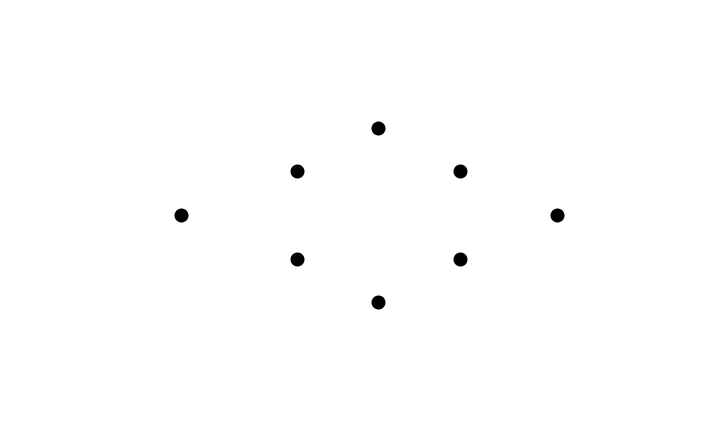
\includegraphics[width=1.00\linewidth]{pics/complexP.png} \\ a. Cloud of points $P$}
\end{minipage}
\begin{minipage}[h]{0.5\linewidth}
\center{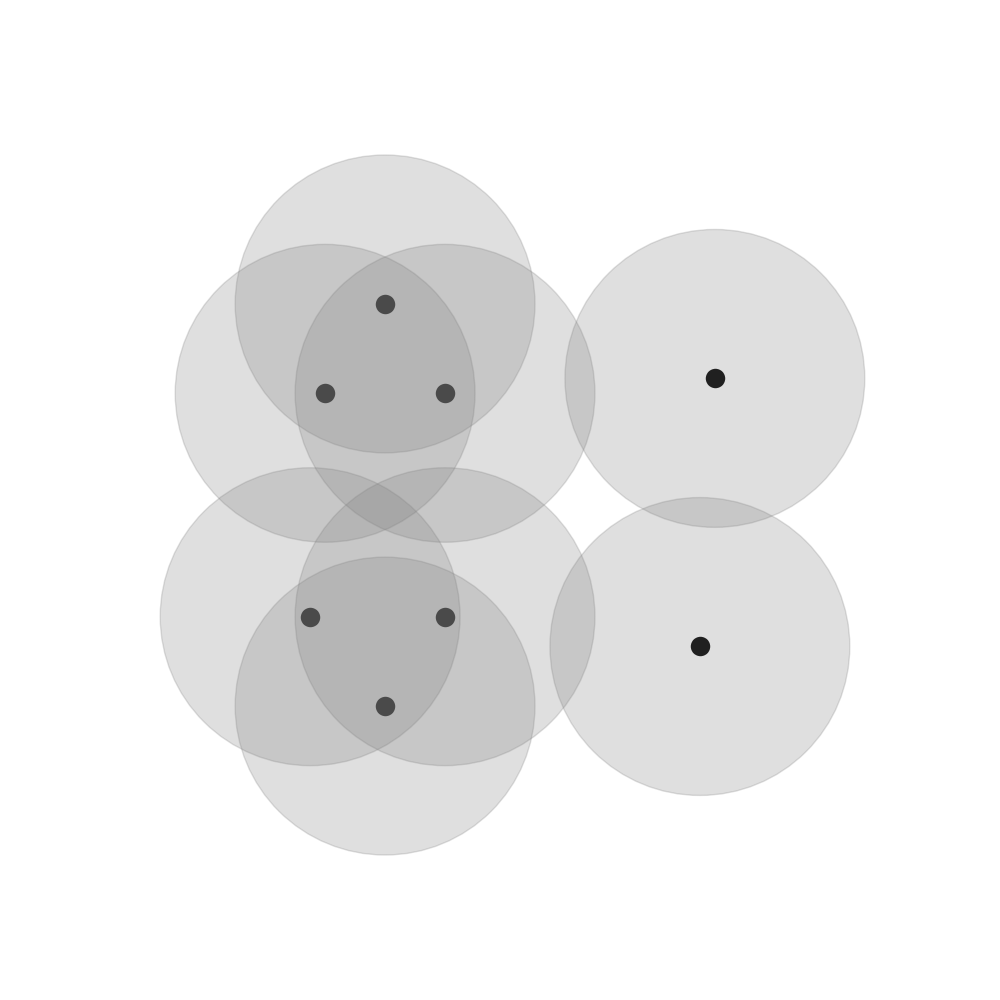
\includegraphics[width=1.00\linewidth]{pics/complexU.png} \\ b. Union of balls $U(P)$}
\end{minipage}
\begin{minipage}[h]{0.5\linewidth}
\center{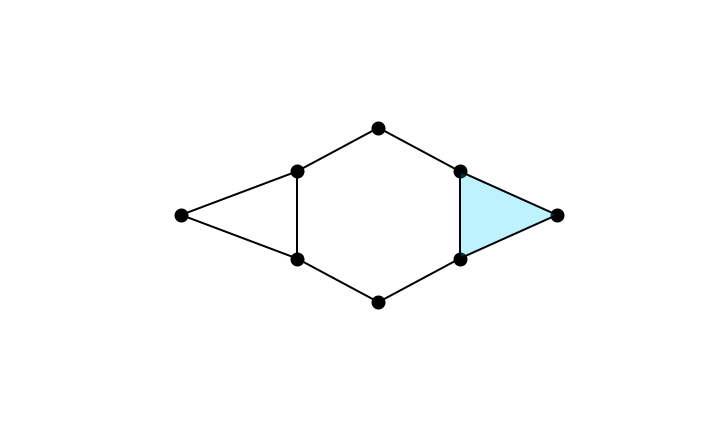
\includegraphics[width=1.00\linewidth]{pics/complexC.png} \\ c. Čech complex $C(P)$}
\end{minipage}
\begin{minipage}[h]{0.5\linewidth}
\center{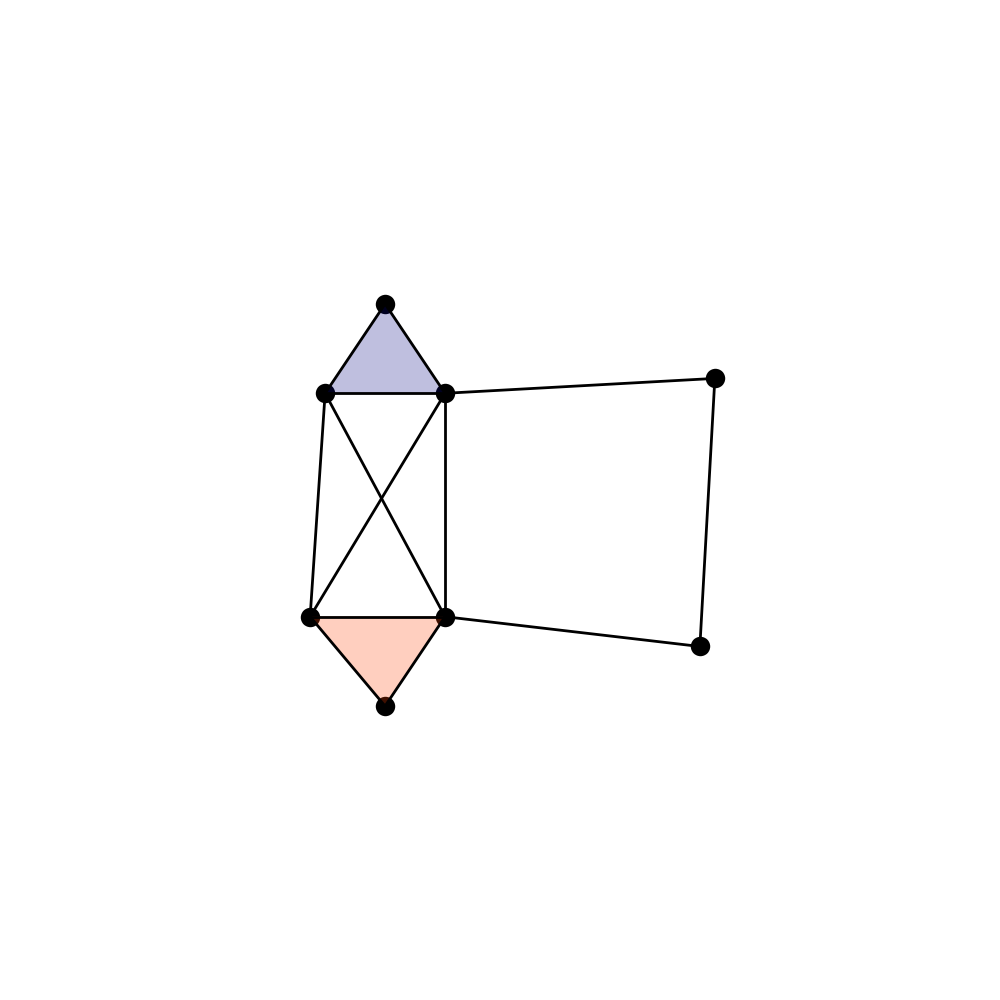
\includegraphics[width=1.00\linewidth]{pics/complexR.png} \\ d. Rips complex $R(P)$}
\end{minipage}
\caption{Demonstration of complexes for some cloud}
\label{image1}
\end{figure}
\par There is associated with Čech complex the union of balls $U(P, r) = \underset{{p\in P}}{\cup}B_r(p)$. That's a completely different structures, but there is a Čech theorem (also known as Nerve theorem), which said, that topologically they are very similar \cite{ghrist}\cite{karol}.
%\par ... (the Čech (Nerve) theorem) 
\par Another one natural method to represent a cloud as a simplicial complex is the Rips complex. For a given cloud $P = \{x_\alpha\}\subset (X, \rho)$ the Rips complex $R_r$ is determined by unordered $(k+1)$-tuples of points whose for each pair of points $\{x_\alpha\}_0^k$ the distance between that pairs points less or equal $r$ \cite{ghrist}.
\par Now we can start to talk about persistent homology. That's one of the popuelar tools used in the field of Applied Topological Data Analysis.
%\par A filtration $\mathbb{X} = \{X_t\}_t$ is a set of topological spaces such that $X_s \subset X_t$ for all $s < t$ \cite{bobprimoz}.%The inclusion maps $i:\; X_s \hookrightarrow X_t$ induce mapping between cycles $i_*:\; H_k(X_s) \to H_k(X_t)$. These maping allow us to track the evolution of cycles: when they start and finish to exist \cite{bobprimoz}.
\par Let us $X$ be some topological space. The filtration of $X$ is the set of topological spaces $\{X_t\}_t$ such that $X_s \subset X_t$ for all $s < t$ \cite{bobprimoz}. Rewriting filtration as $\emptyset = \mathbb{X}_0 \subset \mathbb{X}_1 \subset \cdots \subset \mathbb{X}_m = X$, we can get a linear map for each inclusion
$$
	0 = H(\mathbb{X}_0) \to H(\mathbb{X}_1) \to \cdots \to H(\mathbb{X}_m) \to H(X)
$$
People call the sequences like that persistence modules. Let's split that module into indecomposable sumands like $0 \to F\to\cdots \to F \to 0$, where every nonzero map is the identity. There is a unique such decomposition whose direct sum gives the original module (means which contents all sebsets from a given filtrations). Each summand can be interpreted as the birth of a homology class $H^k$ at its first non-zero term and the death of the same homology class right after its last non-zero term (We will say the birth and the death of $k$-cycle) \cite{morozov}. 
\par The cycles which never dies (there is no non-zero term after birth for them) we will call giant. But that's possible to define them more formal. 
\par Let us $M$ some topological space and $\{X_t\}$ some filtration such that $X_t\subset M \forall t$. For each $t$ the inclusion map $i:\;X_t\hookrightarrow M$ induces a map $i_{*, t}:\; H_k(X_t)\to H_k(M)$. The image of that map $i_{*, t}$ stands for all the cycles that exists in $X_t$ and are mapped to nontrivial cycles in $M$. These are giant cycles \cite{bobprimoz}.

\par Let's throw few examples of persistent homology: we have discussed Cech complex ($C_r$), Reese complex ($R_r$) and associated with the Cech the union of balls $U_r$. So using them we can defind filtrations $\{U_r(P)\}_{r\in\mathbb{R}_+}$, $\{C_r(P)\}_{r\in\mathbb{R}_+}$, $\{R_r(P)\}_{r\in\mathbb{R}_+}$ for a given cloud $P\subset X$, where $X$ is some metric space. You can see example in Figure \ref{image2}.
% picture
\begin{figure}[h!]
\begin{minipage}[h]{1.10\linewidth}
\center{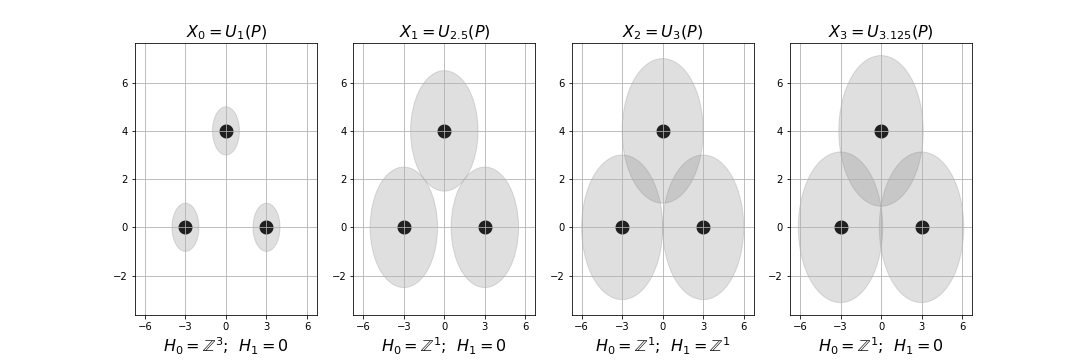
\includegraphics[width=0.97\linewidth]{pics/persistentU.png} \\ a. Filtration $\{U_r(P)\}_{r>0}$}
\end{minipage}
\begin{minipage}[h]{1.10\linewidth}
\center{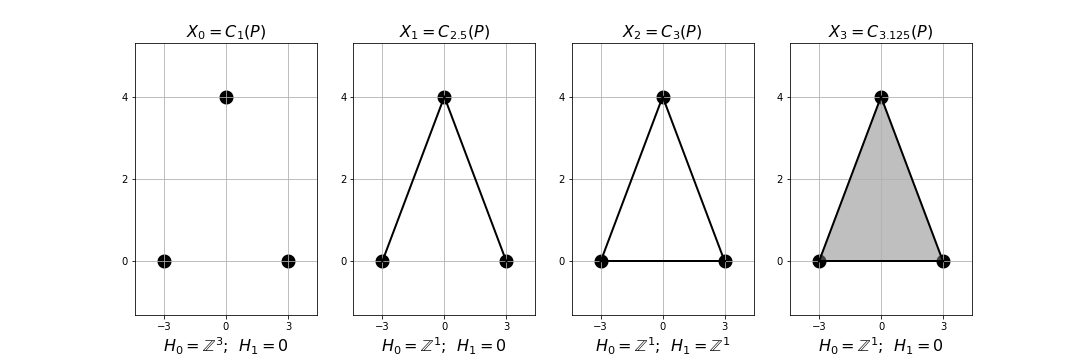
\includegraphics[width=0.97\linewidth]{pics/persistentC.png} \\ b. Filtration $\{C_r(P)\}_{r>0}$}
\end{minipage}
% add Reeze
\caption{There are filtrations $\{U_r(P)\}_{r>0}, \{C_r(P)\}_{r>0} \subset{\mathbb{R}^2}$ where $P=\{(-3, 0), \; (3, 0), \; (0, 4)\}$. In pictures a and b tou can see that filtrations for parameters $r\in\{1,\; 2.5,\; 3,\; 3.125\}$. All them except the first are birth or death values.}
\label{image2}
\end{figure}
\par ...% about barcodes
% picture about barcodes for same cloud as in fig2

\subsection{Lattices, Voronoi Cells and their Extropolation on Torus}
\par In this chapter we will show default definitions about lattices in $\mathbb{R}^n$, talk about Voronoi cells and then extropolate their definitions to the torus case. 
\par A lattice in $\mathbb{R}^n$ is a subset $\Gamma\subset\mathbb{R}^n$ with the property that there exists a basis $(e_1, ..., e_n)$ of $\mathbb{R}^n$ s.t. $\Gamma = \mathbb{Z}e_1 \oplus\cdots\oplus \mathbb{Z}e_n$. The fundamental parallelotope of lattice $\Gamma$ is $\{\lambda_1e_1 + \cdots + \lambda_n e_n \mid 0\le\lambda_i\le1\}$.
\par The matrix with lines $e_1, ..., e_n$ is called generator matrix of lattice $\Gamma$.The matrix of scalar products
$$
G = 
\begin{pmatrix}
	\langle e_1, e_1\rangle & \langle e_1, e_2\rangle & \langle e_1, e_n\rangle \\
	\langle e_2, e_1\rangle & \langle e_2, e_2\rangle & \langle e_2, e_n\rangle \\
	\cdots & \cdots & \cdots & \cdots \\
	\langle e_n, e_1\rangle & \langle e_n, e_2\rangle & \langle e_n, e_n\rangle
\end{pmatrix}
$$
is known as Gram matrix \cite{ebeling}.
\par If one lattice can be obtained from another by (possibly) a rotation, reflection and change of scale we say they are equivalent. More formally two lattices with generator matrices $G$ and $G'$ are equivalent, if and only if $G' = cUMB$, where $c$ is some nonzero constant, $U$ is a matrix with integer entries s.t $|\det U| = 1$ and B is a real orthogonal matrix. The corresponding Gram matrices are relited by $A' = c^2UAU^{T}$ \cite{conway}.
\par The binary operation for two vectors $\alpha, \beta$ $S_\alpha(\beta)$ is called reflection if $S_\alpha(\alpha) = -\alpha$ and $S_\alpha(\beta) = \beta$ for each $\beta\perp\alpha$. 
Usually $S_\alpha(\beta) = \beta - 2\cfrac{\langle\lambda, \beta\rangle}{\langle\lambda, \alpha\rangle}\alpha$. 
\par The finite set of vetcors $\Phi$ is a root system if $\Phi\cap\mathbb{R}\alpha = \{\alpha, -\alpha\}$ and $S_\alpha\Phi = \Phi$ for each $\alpha$ from $\Phi$ \cite{smirnov}.
\par The lattices generated by root systems called root lattices.
\par Let's throw few examples of lattices, which will be interesting in this work. That's root lattices.
\par The Lattice $\mathbb{Z}^n$ is the most simpliest lattice, that's just the set of all vectors from $\mathbb{R}^n$ which all elements are integer.
$$
	\mathbb{Z}^n = \{(x_1, ..., x_n):\; x_i\in\mathbb{Z}\} \subset \mathbb{R}^n
$$
That's generator matrix and Gram matrix is identity matrix $\mathbb{I}_n$. 
\par The Lattice $A_n$ ($n \ge 1$) is the subgroup of lattice $\mathbb{Z}^{n+1}$ which elements lie on the hyperplane $\sum\limits_{i=0}^n x_i = 0$.
$$
	A_n = \{(x_1, x_1, ..., x_n)\in \mathbb{Z}^n:\; x_1 + \cdots x_n = 0\}
$$
That's generator matrix can look like that:
$$
M_{A_n} = 
\begin{pmatrix}
	-1 & 1 & 0 & 0 & \cdots & 0 & 0 \\
	0 & -1 & 1 & 0 & \cdots & 0 & 0 \\
	0 & 0 & -1 & 1 & \cdots & 0 & 0 \\
	\cdots & \cdots & \cdots & \cdots & \cdots & \cdots & \cdots \\
	0 & 0 & 0 & 0 & \cdots & -1 & 1 
\end{pmatrix}
$$
And there are two types of gram matrices possible:
$$
\begin{pmatrix}
	2 & -1 & 0 & \cdots & 0 & 0 \\
	-1 & 2 & -1 & \cdots & 0 & 0 \\
	0 & -1 & 2 & \cdots & 0 & 0 \\
	\cdots & \cdots & \cdots & \cdots & \cdots & \cdots \\
	0 & 0 & 0 & \cdots & 2 & -1 \\
	0 & 0 & 0 & \cdots & -1 & 2 
\end{pmatrix}
$$
or
$$
\begin{pmatrix}
	2 & 1 & 1 & \cdots & 1 & 1 \\
	1 & 2 & 1 & \cdots & 1 & 1 \\
	1 & 1 & 2 & \cdots & 1 & 1 \\
	\cdots & \cdots & \cdots & \cdots & \cdots & \cdots \\
	1 & 1 & 1 & \cdots & 2 & 1 \\
	1 & 1 & 1 & \cdots & 1 & 2 
\end{pmatrix}
$$
\par The Lattice $D_n$ can be defined for $n \ge 3$. That's the subgroup of $\mathbb{Z}^n$ consists all elements which sum coefficients is even.
$$
	D_n = \{(x_1, ..., x_n)\in \mathbb{Z}^n:\; x_1 + \cdots + x_n \mid 2\}
$$
That's generator matrix can look like that :
$$
M_{D_n} = 
\begin{pmatrix}
	-1 & -1 & 0 & 0 & \cdots & 0 & 0 \\
	-1 & 1 & 0 & 0 & \cdots & 0 & 0 \\
	0 & -1 & 1 & 0 & \cdots & 0 & 0 \\
	0 & 0 & -1 & 1 & \cdots & 0 & 0 \\
	\cdots & \cdots & \cdots & \cdots & \cdots & \cdots & \cdots \\
	0 & 0 & 0 & 0 & \cdots & -1 & 1 
\end{pmatrix}
$$
and that's Gram matrix:
$$
\begin{pmatrix}
2 & 2 & 0 & \cdots & 0 & 0 \\
2 & 2 & -1 & \cdots & 0 & 0 \\
0 & -1 & 2 & \cdots & 0 & 0 \\
\cdots & \cdots & \cdots & \cdots & \cdots & \cdots \\
0 & 0 & 0 & \cdots & 2 & -1 \\
0 & 0 & 0 & \cdots & -1 & 2 \\ 
\end{pmatrix}
$$
\par People also call that lattice checkerboard lattice \cite{conway}.
\par That's easy to see, that's $A_3 \equiv D_3$, cause by permutations of vectors in $M_{A_3}$ and calculating corresponding Gram matrix we will get the Gram matrix of $D_3$:
$$
\begin{pmatrix}
	2 & -1 & 0 \\
	-1 & 2 & -1 \\
	0 & -1 & 2
\end{pmatrix}
$$


\par Let's define a lattice $\Gamma^*$ dual to $\Gamma$ as $\{x\in\mathbb{R^n} :\; x\cdot y\in\mathbb{Z} \; \forall y\in\Gamma\}$ \cite{ebeling}.
\par That's easy to understand, that lattice $\mathbb{Z}^n$ is self-dual (self-dual lattice is the lattice $\Gamma$ such that $\Gamma^* = \Gamma$)
\par The lattice $A_n^*$ dual to $A_n$ has folows generator matrix
$$
M_{A_n^*} = 
\begin{pmatrix}
	1 & -1 & 0 & \cdots & 0 & 0 \\
	1 & 0 & -1 & \cdots & 0 & 0 \\
	\cdots & \cdots & \cdots & \cdots & \cdots & \cdots \\
	1 & 0 & 0 & \cdots & -1 & 0 \\
	\cfrac{-n}{n+1} & \cfrac{1}{n+1} & \cfrac{1}{n+1} & \cdots & \cfrac{1}{n+1} & \cfrac{1}{n+1}
\end{pmatrix}
$$
And the related to that definition Gram matrix will be
$$
\begin{pmatrix}
	n & -1 & -1 & \cdots & -1 \\
	-1 & n & -1 & \cdots & -1 \\
	\cdots & \cdots & \cdots & \cdots & \cdots \\
	-1 & -1 & -1 & \cdots & n
\end{pmatrix}
$$
That's not hard to check that $M_{A_n}\cdot M_{A_n^*}^T = \mathbb{I}_n$.
\par The generator matrix of lattice $D_n^*$ dual to $D_n$ will be
$$
M_{D_n^*} = 
\begin{pmatrix}
1 & 0 & \cdots & 0 & 0 \\
0 & 1 & \cdots & 0 & 0 \\
\cdots & \cdots & \cdots & \cdots & \cdots \\
0 & 0 & \cdots & 1 & 0 \\
\cfrac{1}{2} & \cfrac{1}{2} & \cdots & \cfrac{1}{2} & \cfrac{1}{2} 
\end{pmatrix}
$$
\par $D_3^*$ is the body centered cubic lattice, like $A_3^*$, and $D_4^* \equiv D_4$ \cite{conway}.
\par ... % Voronoi

\par Let's define $d$-dimensional torus as $\mathbb{R}^n/\mathbb{Z}^n$ or $\left(\mathbb{R}/\mathbb{Z}\right)^n$ (Omer Bobrowski and Shmueluse Weinberger use that definition in \cite{vanish}). Not hard to see, that $\mathbb{R}/v_1\mathbb{Z}\times\cdots\times\mathbb{R}/v_n\mathbb{Z}$ ($v_1,..., v_n\in\mathbb{R}_{>0}$) will be the homeomorphically-same object.
\par Let's redefine lattice thinking, they lie not just on $\mathbb{R}^n$, but on some torus with defined equivalence relation given by vector $v = (v_1, ..., v_n)\in \mathbb{R}^n_{>0}$: for $a, b\in \mathbb{R}$ $a \equiv b$ if $a-b = vk$ $k\in\mathbb{Z}$. That's litterally equivalence relation from the given torus definition. If for the lattice basis $e_1, ..., e_n$ and the given vector $v$ and eacn $k\in\{1, ..., n\}$ there exists $j\in\mathbb{Z}$ s.t. $jv_k \mid {e_i}_k$ the lattice will have finite number of elemens on torus defined by vector $v$.
\par ...% notation

\section{...}
\subsection{Percoation on Cells}
\par Continuum-percolation models are random processes in which subsets $D_i \subseteq X$ where $i\in\{1, ..., N\}$ are chosen randomly with some probability distribution in a structure $\underset{i=1}{\overset{N}{\cup}} D_i$ \cite{percolationdisks}.
\par ...


\newpage
\addcontentsline{toc}{section}{References}
\begin{thebibliography}{}
\bibitem{karol} Karol Borsuk. (1948) On the imbedding of systems of compacta in simplicial complexes. Fundamenta Mathematicae, 35(1):217–234, 1948.
\bibitem{conway} Conway, John \; Sloane, N.. (1988). Sphere Packings, Lattices and Groups. 10.1007/978-1-4757-2016-7. 
\bibitem{hatcher} Hatcher, A. (2001). Algebraic topology. Proceedings of The Edinburgh Mathematical Society - PROC EDINBURGH MATH SOC. 46. 511-512. 10.1017/S0013091503214620. 
\bibitem{ebeling} Ebeling, Wolfgang. (2002). Lattices and Codes. 10.1007/978-3-322-90014-2.
%\bibitem{zamorodian} A. Zomorodian and G. Carlsson, “Computing persistent homology”, Discrete Comput. Geom., 33 (2005), 249–274. MR2121296 (2005j:55004)
\bibitem{prasolov}  Prasolov, V. V. (2006), Elements of combinatorial and differential topology, American Mathematical Society, ISBN 0-8218-3809-1, MR 2233951
\bibitem{ghrist} Ghrist, Robert. (2008). Barcodes: The persistent topology of data. BULLETIN (New Series) OF THE AMERICAN MATHEMATICAL SOCIETY. 45. 10.1090/S0273-0979-07-01191-3. 
\bibitem{morozov} Edelsbrunner, Herbert \; Morozov, D.. (2012). Persistent homology: Theory and practice. Proceedings of the European Congress of Mathematics. 31-50. 
\bibitem{vanish} Bobrowski, Omer \; Weinberger, Shmuel. (2015). On the Vanishing of Homology in Random Čech Complexes. Random Structures and Algorithms. 10.1002/rsa.20697. 
\bibitem{smirnov} Е.Ю. Смирнов ”Группы отражений и правильные многогранники” Издание
второе, исправленное и дополненное. Москва. МЦНМО. 2018.
\bibitem{percolationdisks} Speidel, Leo \; Harrington, Heather \; Chapman, Stephen \; Porter, Mason. (2018). Topological data analysis of continuum percolation with disks. Physical Review E. 98. 10.1103/PhysRevE.98.012318. 
\bibitem{bobprimoz} Bobrowski, Omer \; Skraba, Primoz. (2019). Homological Percolation and the Euler Characteristic. 
\end{thebibliography}




\end{document}